\setchapterpreamble[u]{
    \dictum[Bob Kahn en \textit{Where Wizards Stay Up Late}]{\textquote{It’s one thing when you plug in to a socket in the wall and electrons flow. It’s another thing when you have to figure out, for every electron, which direction it takes.}}
}
\chapter{Resultados de la síntesis del SweRV-EL2 y NoC}

Aunque el objetivo principal del proyecto es realizar un diseño RTL, se ha sintetizado dicho diseño para la plataforma objetivo Virtex-7 VC707 Evaluation Kit, que hace uso de una FPGA Virtex-7 XC7VX485T-2FFG1761C \cite{XilinxVC707}.

Esta FPGA cuenta con 700 pines de entrada/salida, más de 300 mil LUTs y 600 mil registros.

\section{Área utilizada por el diseño}
Se ha generado un reporte de utilización usando Xilinx Vivado tras sintetizar para la Virtex-7 con la configuración por defecto. Debido a que aún no se ha realizado la fase de implementación ni sus optimizaciones, estos resultados son una mera estimación, pudiendo ser diferentes al realizar el flujo de implementación a la FPGA.

En total, el diseño sintetizado (que incluye \textit{core}, memoria e interfaz DMI) ocupa un $14\%$ de las LUTs de la FPGA (40 mil), y un $4\%$ de sus registros (23 mil), siendo con diferencia el \textit{core} el que más área consume: un $12\%$ y $3.59\%$ de los recursos disponibles en la FPGA respectivamente (36 mil y 21 mil).

Dentro del \textit{core}, su elemento más pesado es la IFU, con 11 mil LUTs ($3.69\%$), seguido de la EXU con 10 mil LUTs ($3.18\%$). Por lo tanto, solo estos dos elementos ya forman el 40\% de los LUTs consumidos por el core, dejando un $3.77\%$ del total (11 mil LUTs) para el DEC y el LSU. Por otra parte, dos tercios de los registros del \textit{core} son utilizados por el IFU. En la figura \ref{fig:plots_area_core} se visualizan dichos áreas. Todos los \textit{senders} y \textit{receivers} instanciados a este nivel (es decir, sin contar los de dentro de los wrappers) sumados hacen uso de 66 LUTs y 79 flip-flops, siendo los receptores los que más registros consumen (70 de los 79), puesto que deben almacenar los datos del paquete recibido. El detector de reloj ha sido sintetizado a un flip-flop.
\begin{figure}[h]
    \centering
    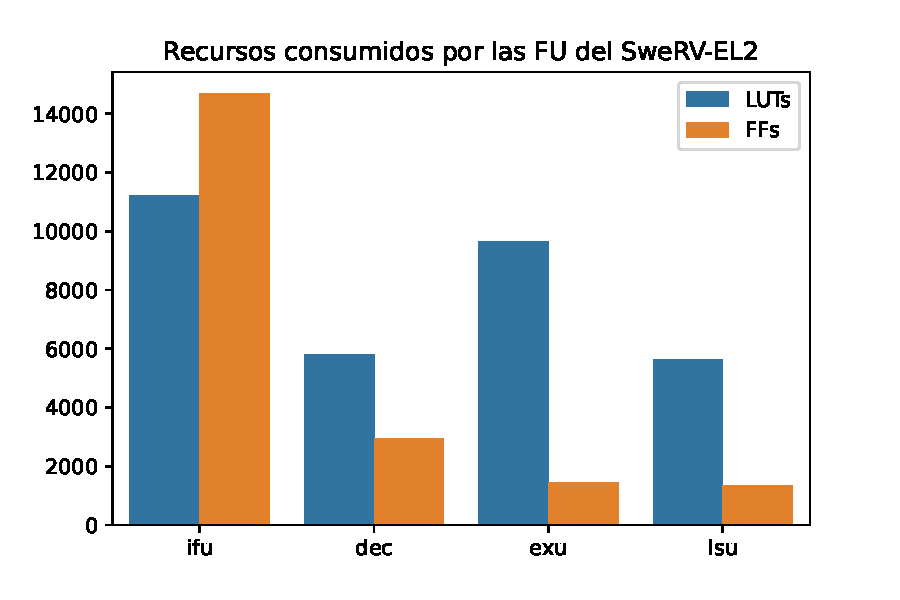
\includegraphics[width=12cm]{images/plots/swerv_fu.pdf}
    \caption[Recursos consumidos por las unidades funcionales del \textit{core}.]{Recursos consumidos por las unidades funcionales del \textit{core}.}
    \label{fig:plots_area_core}
\end{figure}

\subsection{Recursos utilizados en la unidad de ejecución y la NoC}
A continuación analizaremos el uso de recursos de la EXU, a la que se le ha incluido una NoC. 
En la figura \ref{fig:plots_area_exu} se visualizan los datos mencionados a continuación.
De los 9700 LUTs usados por la EXU, 2700 ($28\%$) son ocupados por los encaminadores y conexiones de la NoC. A los wrappers del multiplicador y el divisor se les asignan 1433 y 744 LUTs respectivamente. Otra gran parte de los recursos de la EXU (2214 LUTs, $23\%$) son asignados al módulo \textit{i\_x\_ff}, encargado de parte de la lógica de predicción de salto.

\begin{figure}[p]
    \centering
    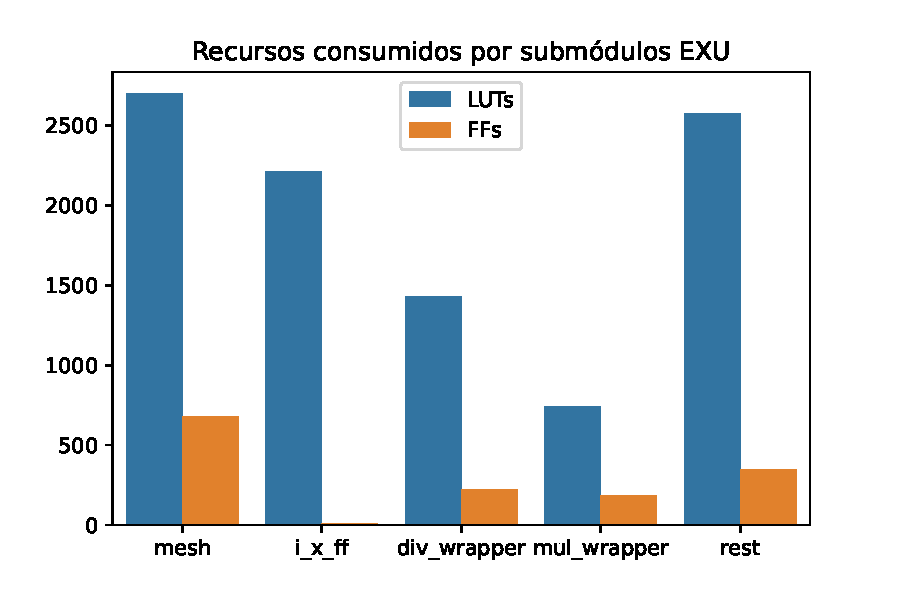
\includegraphics[width=13cm]{images/plots/swerv_exu.pdf}
    \caption[Recursos consumidos por los submódulos de la unidad de ejecución.]{Recursos consumidos por los submódulos de la unidad de ejecución. En rest se muestran los LUTs y \textit{flip-flops} utilizados tanto para el resto de submódulos de la EXU como para la lógica y conexiones del módulo EXU.}
    \label{fig:plots_area_exu}
\end{figure}

\begin{figure}[p]
    \centering
    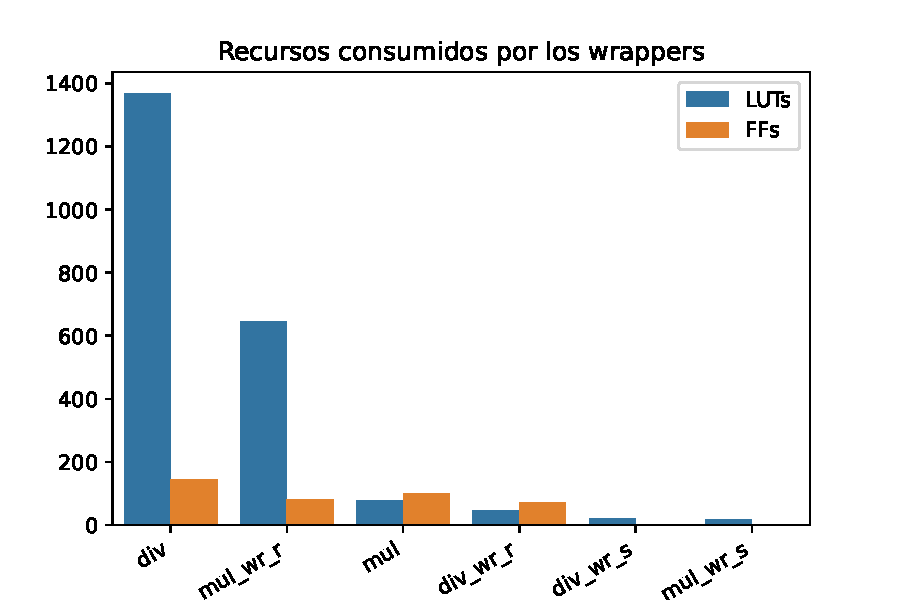
\includegraphics[width=13cm]{images/plots/swerv_wrappers.pdf}
    \caption[Recursos consumidos por los \textit{wrappers} de los submódulos de la EXU.]{Recursos consumidos por los \textit{wrappers} de los submódulos de la EXU.}
    \label{fig:plots_area_wrappers}
\end{figure}

Finalmente, analizaremos los recursos consumidos por los \textit{wrappers}, para discernir si su tamaño es debido a las unidades de cálculo (el multiplicador y el divisor en sí), o por los elementos adicionales (emisores y receptores). Se presentan una visualización de los datos en la figura \ref{fig:plots_area_wrappers}. En cuanto al divisor, su \textit{wrapper} ocupa en total 1433 LUTs, y 1368 de estos son para el submódulo divisor, por lo que los elementos adicionales de comunicación de la red emplean tan solo 65 LUTs (un 5\% del wrapper). Por otro lado, el envoltorio del multiplicador ocupa un total de 744 LUTs, mientras que su submódulo principal tan solo cuenta con 79 de estos, dejando que los dispositivos de red utilicen 665 LUTs, el 90\% del wrapper. Esto es debido a que el receptor tiene un gran tamaño, empleando 646 LUTs (86\% del wrapper).
% \tdinquiry{Ocupa un montón el receptor... ¿Eso lo digo? Tampoco sé muy bien por qué ocurre...}

Para concluir, comprobaremos qué parte de los recursos de la  EXU son consumidos por los módulos añadidos. Si sumamos los recursos consumidos por todos ellos (malla y emisores/receptores, tanto dentro como fuera de \textit{wrappers}), tenemos que se han añadido 3496LUTs y 918 FFs, principalmente debido a la malla (2700LUTs y 678FFs). Estos elementos son el 36\% de los LUTs y el 63\% de los \textit{flip-flops} de la EXU. Es decir, la inserción de la NoC ha aumentado el número de LUTs consumidos por la EXU en 57\%, y el de registros en 174\%. En conclusión, la NoC tan solo ha aumentado el tamaño total del diseño en un 9\% de LUTs y un 4\% de FFs.

% \tdinquiry[inline, caption={Cosas por hacer reportes}]{
% \begin{itemize}
%     \item Hablar de la FPGA objetivo y sus características
%     \item Área
%     \item En conclusión... las cosas añadidas suman nosecuantas LUTs y registros
% \end{itemize}
% }
